\section{Vorstellung Prototyp}
Nachfolgend folgt die Vorstellung des GUI-Prototypen zum Business Transformation Tracker. Da dieser als Webanwendung konzeptiert ist, wurde auch der GUI-Protoyp an eine Webanwendung angelehnt. Der Prototyp erfüllt den Zweck die analysierten Anforderungen in einer grafischen Benutzeroberfläche abzubilden, um dem Auftraggeber und den Anwendern erste, leicht verständliche Einblicke das OOA-Modell zu geben. Dieser Prototyp dient bei einer späteren Umsetzung und Implementierung des BBT als Vorlage für die Benutzeroberfläche.

\subsubsection{Verwendete Werkzeuge}
Für die Entwicklung des Prototypen wurde auf das Programm Adobe XD zurück-gegriffen. Dies entstammt dem Softwarehersteller Adobe und ist Teil der Softwaresuite \glqq{}Creative Cloud\grqq{}. Das Programm ist nur in einem Abonnement erhältich und kostet etwa 12 Euro im Monat. Adobe XD ist eine Grafiksoftware mit der sich komplexe, grafische Benutzeroberflächen für unterschiedliche Bildschirmgrößen gestalten und animieren.\footcite[Vgl.][]{adobe} Auf die Animationsfunktion wurde jedoch nicht zurückgegriffen.

\subsubsection{Aufbau der Benutzeroberfläche}
Der Aufbau des Prototypen beginnt mit der Login-Fläche, die in Abbildung \ref{fig:Login} dargestellt ist. Auf dieser muss sich der Benutzer, im Falle einer späteren Implementierung, mit seinem persönlichen Benutzernamen und Kennwort anmelden.
\begin{figure}[h!]
    \centering
    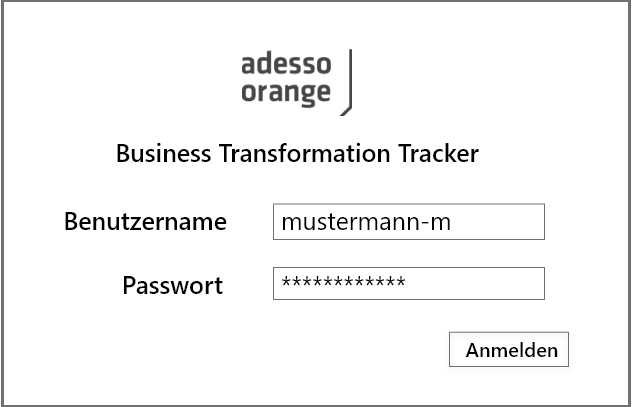
\includegraphics[scale=0.35]{./Prototyp/01_Login.png}
    \caption[Prototyp: Login-Bildschirm]{Login-Bildschirm}
    \label{fig:Login}
\end{figure}
\\Nachdem diese Anmeldung erfolgreich war, findet sich der Anwender auf der Startseite wieder, auf der er aktuelle Informationen über den Business Transformation Tracker und adesso orange vorfindet.
Auch sieht er hier zum ersten Mal den Aufbau, der sich durch die gesamte Benutzeroberfläche hindurchzieht. Bei der Gestaltung der Oberfläche wurde auf ein \glqq{}Kachel-Design\grqq{} mit großen Schaltflächen gesetzt, sodass die Oberfläche auch auf mobilen Endgeräten einfach zu verwenden ist. Bei der Farbgebung wurde sich an den Design-Farben von adesso orange orientiert. Die Bedeutung der unterschiedlichen Farben in den Kacheln wird später erläutert. 
\begin{figure}[h!]
    \centering
    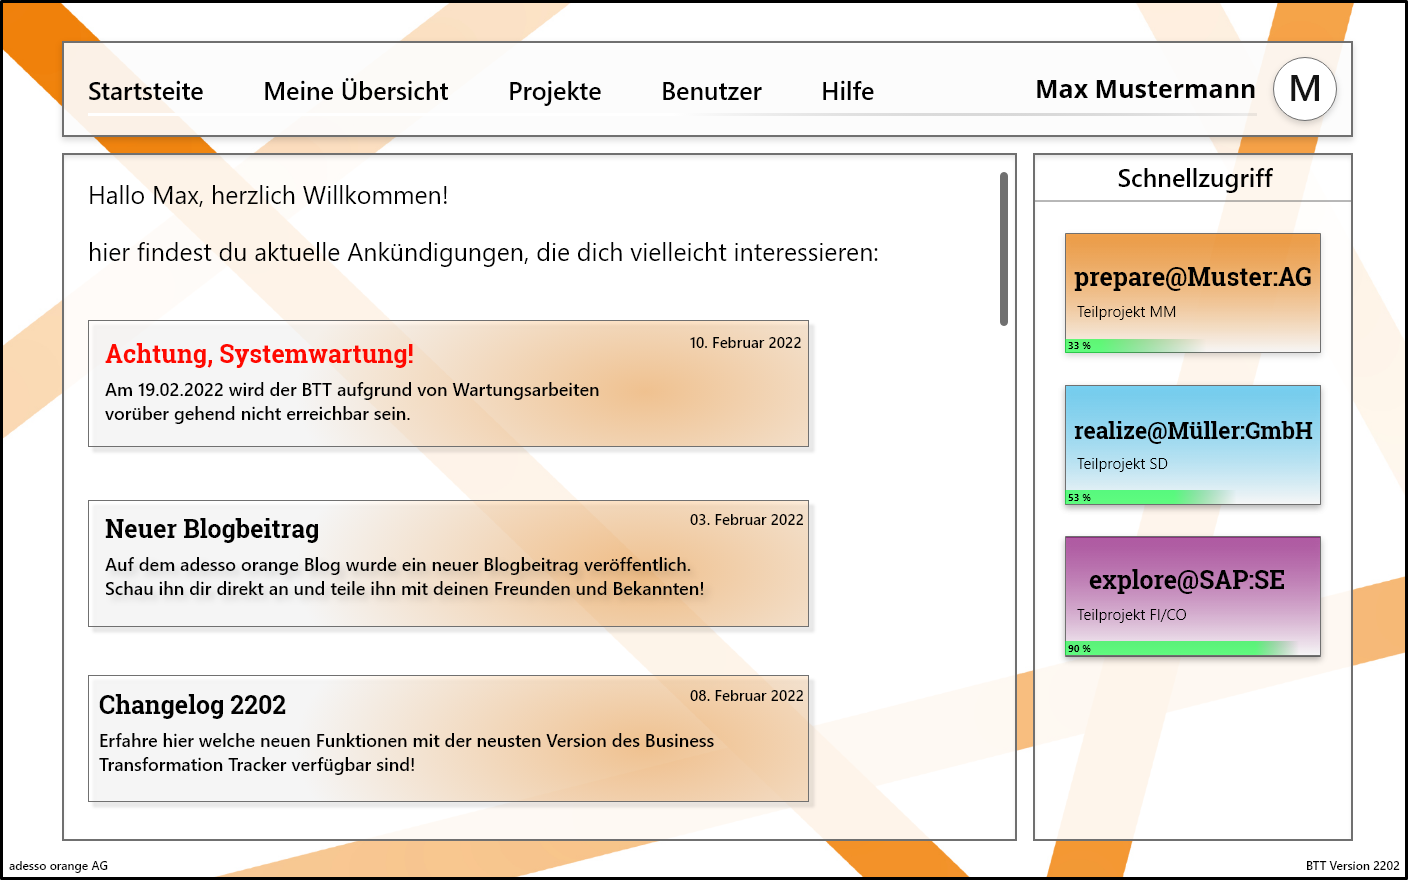
\includegraphics[scale=0.35]{./Prototyp/02_Startseite.png}
    \caption[Prototyp: Startseite]{Startseite}
    \label{fig:Startseite}
\end{figure}
\\Wie in Abbildung \ref{fig:Startseite} zu sehen, befindet sich im Kopf der Oberfläche eine Menüleiste wieder, von der aus der Benutzer schnellen Zugriff auf wichtige Funktionen erhält. Mit dem Punkt \glqq{}Startseite\grqq{} gelangt er auf die hier dargestellte Startseite, mit dem Punkt \glqq{}Meine Übersicht\grqq{} auf eine Übersicht, in der er die ihm zugeordneten Projekte sehen kann, über den Menüpunkt \glqq{}Projekte\grqq{} und \glqq{}Benutzer\grqq{} jeweils auf die Projekt- und die Benutzerübersicht. Die Besonderheit an den letzten beiden Punkten ist, dass sie nur für die Rollen der Projektleiter und Administratoren sichtbar sind, damit nicht jeder Zugriff auf die Benutzer, und somit den personenbezogenen Daten, und allen anderen Projekte erhält. Als Letztes befindet sich in der Menüzeile der Punkt \glqq{}Hilfe\grqq{}, mit dem der Benutzer später auf die Anwenderdokumentation zugreifen kann, sowie sein eigener Name und Platz für ein Profilbild.\\Auf der rechten Seite befindet sich, abgetrennt vom breiten Hauptfenster, ein schmaleres Fenster mit der Überschrift Schnellzugriff. In diesem werden dem Benutzer die ihm zugordneten Projekte angezeigt, sowie das ihm zugeordnete Teilprojekt und der aktuelle Fortschrittsgrad von diesem. Der Name der Projekte setzt sich aus der aktuellen Projektphase und dem Namen des Kunden zusammen.
\begin{figure}[h!]
    \centering
    \includegraphics[scale=0.35]{./Prototyp/031_Projektübersicht.png}
    \caption[Prototyp: Projektübersicht]{Projektübersicht}
    \label{fig:Projektübersicht}
\end{figure}
\\In Abbildung \ref{fig:Projektübersicht} wird die Projektübersicht gezeigt, in die man gelangt, wenn man in der Menüzeile auf \glqq{}Projekte\grqq{} klickt. Hier sind alle im System angelegten Projekte zu sehen, geordnet nach Projektphase. Die Projekte sind auch hier wieder durch Kacheln dargestellt, die neben dem Projektnamen und dem Fortschrittsgrad, auch die Anzahl der Teilprojekte und die zugeordneten Mitarbeiter enthalten. Die Kacheln sind unterschiedlich, nach Projektphase gefärbt, sodass immer auf einem Blick zu erkennen ist, in welcher Phase sich das Projekt momentan befindet. Im schmalen, rechten Fenster befindet sich wieder der Schnellzugriff, mit dem man hier die Projekte nach Projektphase filtern kann. In der oberen, rechten Ecke des Hauptfensters befindet sich ein Button mit dem ein neues Projekt hinzugefügt werden kann.
\begin{figure}[h!]
    \centering
    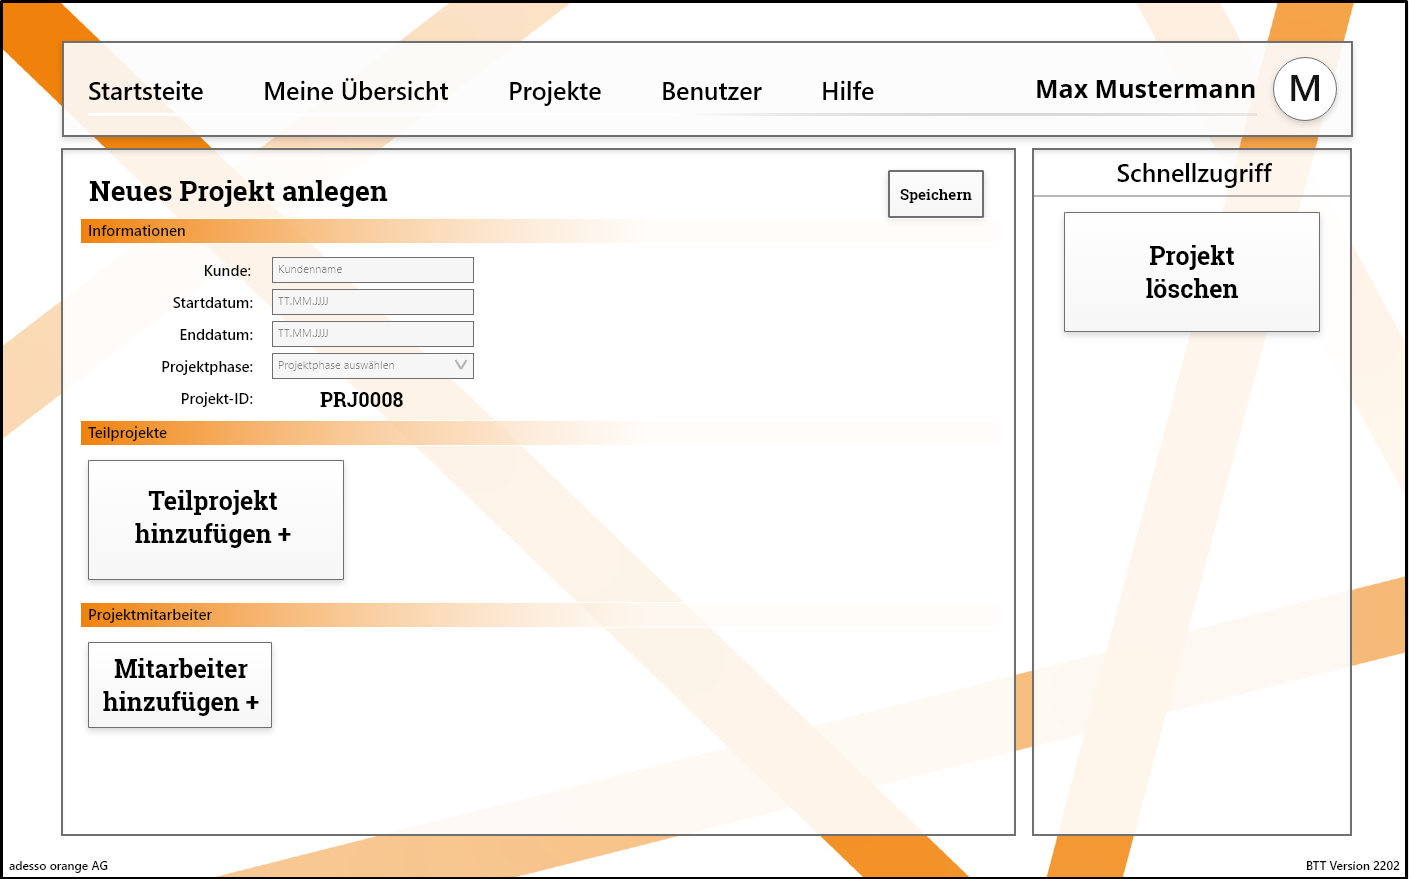
\includegraphics[scale=0.35]{./Prototyp/042_Projekt bearbeiten.png}
    \caption[Prototyp: Projekt anlegen]{Projekt anlegen}
    \label{fig:ProjektAnlegen}
\end{figure}
\\In Abbildung \ref{fig:ProjektAnlegen} ist das Ergebnis der Button-Betätigung zu sehen. In dieser Ansicht kann der Benutzer ein neues Projekt anlegen. Dazu gibt er die Stammdaten des Projekts an und kann danach im unteren Bereich Teilprojekte und Benutzer hinzufügen. Die Projekt-ID wird automatisch vergeben. Nach dem Klick auf \glqq{}Speichern\grqq{} wird das Projekt im System angelegt. 
\begin{figure}[h!]
    \centering
    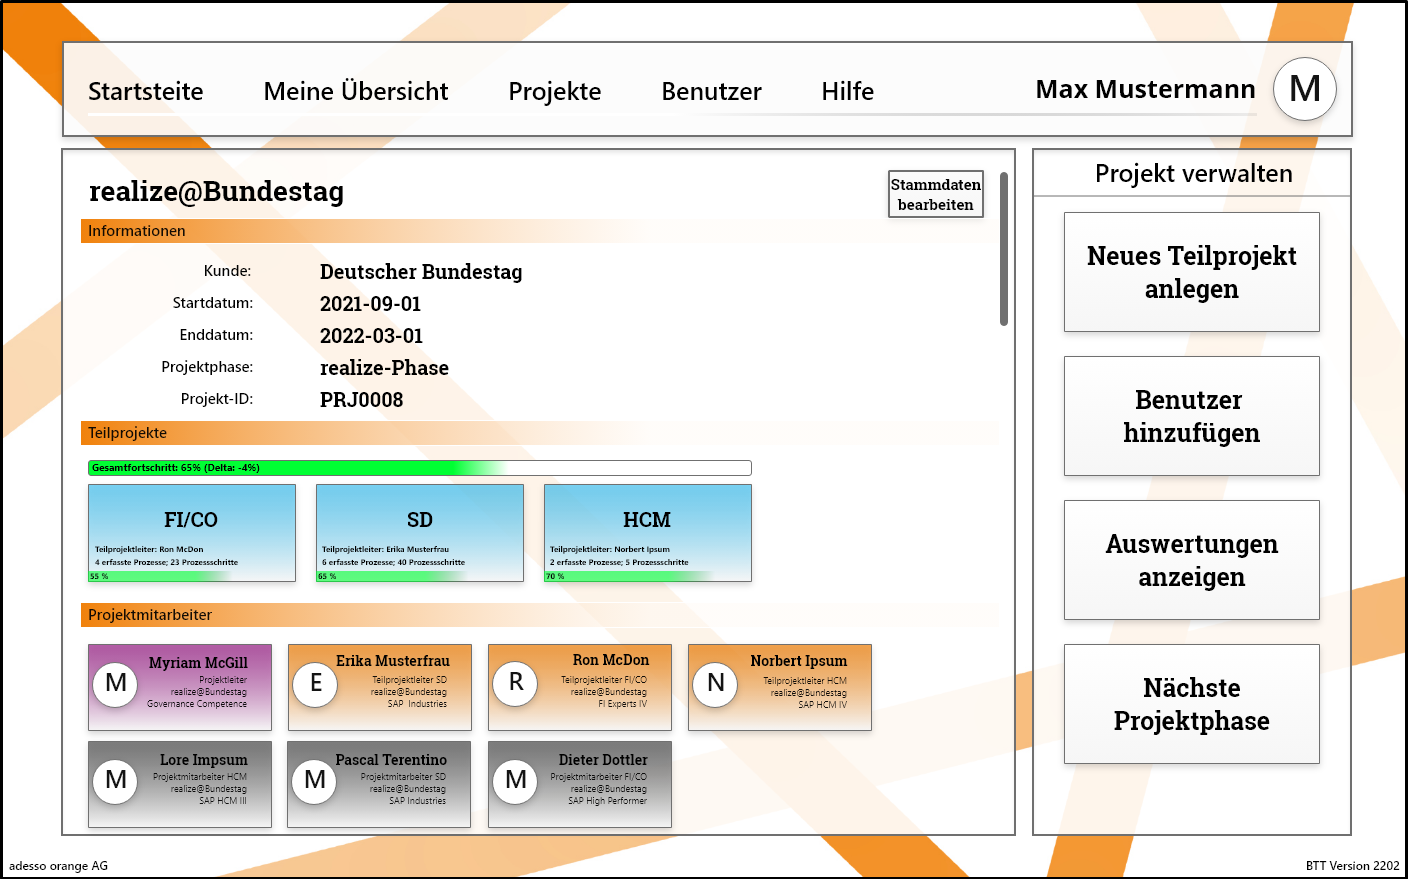
\includegraphics[scale=0.35]{./Prototyp/041_Projekt Ansicht.png}
    \caption[Prototyp: Projektansicht]{Projektansicht}
    \label{fig:Projektansicht}
\end{figure}
\\In Abbildung \ref{fig:Projektansicht} ist ein angelegtes Projekt zu sehen, das bereits seit längerem in Arbeit ist. Im oberen Bereich des Hauptfensters sieht der Benutzer die Stammdaten des Projekts, darunter die vorhandenen Teilprojekte und unten die zugeordneten Projektmitarbeiter. Die Mitarbeiter sind ebenfalls durch farbige Kacheln dargestellt, die Aussagen über ihre Projektrolle, ihr Teilprojekt, sowie ihre Abteilung machen. Auch in dieser Ansicht lassen sich die Fortschrittsgrade der Teilprojekte begutachten, sowie oberhalb der Teilprojekte, den des Projekts. Im Schnellzugriff befinden sich hier verschiedene Möglichkeiten, das Projekt zu verwalten.
\begin{figure}[h!]
    \centering
    \includegraphics[scale=0.35]{./Prototyp/051_Teilprojekt Übersicht.png}
    \caption[Prototyp: Teilprojekt Übersicht]{Teilprojekt Übersicht}
    \label{fig:TeilprojektÜbersicht}
\end{figure}
\\Mit einem Klick auf eine der Teilprojektkacheln, gelangt man, wie in Abbildung \ref{fig:TeilprojektÜbersicht} zu sehen, in die Übersicht des Teilprojekts. Hier werden schließlich die erfassten Prozesse abgebildet, die zu Beginn eines Transformationsprojekts aufgenommen wurden. Die einzelnen Prozesse sind durch Abschnitte voneinander getrennt und die jeweiligen Prozessschritte wiederum durch Kacheln dargestellt. Die Prozesschritt-Kacheln sind nummeriert und tragen jeweils die Überschrift des Schrittes. Ebenfalls zeigen bereits die Kacheln an, wieviele Kriterien des einzelnen Schritts bereits erfüllt sind. Der Benutzer kann über den Schnellzugriff neue Prozesse erfassen oder die Kriterien, die in den Prozesschritten abgefragt werden, verändern.
\begin{figure}[h!]
    \centering
    \includegraphics[scale=0.35]{./Prototyp/061_Kriterien ausfüllen.png}
    \caption[Prototyp: Prozesschritt befüllen]{Prozesschritt befüllen}
    \label{fig:ProzesschrittBefuellen}
\end{figure}
\\Um die Kriterien auszufüllen, reicht ein Klick auf die Kachel eines Prozessschrittes. Daraufhin öffnet sich ein neues Fenster, in dem der Anwender schließlich die Kriterien der aktuellen Projektphase für den oben benannten Prozessschritt ausfüllen kann (siehe Abbildung \ref{fig:ProzesschrittBefuellen}). Die Kriterien der nächsten und der vorherigen Projektphase werden darüber und darunter angezeigt, dort kann der Benutzer jedoch nichts ausfüllen. Um zum nächsten oder zum vorherigen Prozessschritt zu gelangen, genügt ein Klick auf eine der beiden unteren Schaltflächen.
\begin{figure}[h!]
    \centering
    \includegraphics[scale=0.35]{./Prototyp/032_Benutzerübersicht.png}
    \caption[Prototyp: Benutzerübersicht]{Benutzerübersicht}
    \label{fig:Benutzeruebersicht}
\end{figure}
\\Ebenfalls im Prototypen abgebildet ist die Benutzerverwaltung, die in Abbildung \ref{fig:Benutzeruebersicht} dargestellt ist. In dieser finden sich alle im System angelegten Benutzer, nach Rolle sortiert, wieder. Auch die dafür genutzten Kacheln sind wieder farblich gekennzeichnet. Administratoren tragen die Farbe Blau, Projektleiter die Farbe Violett, Teilprojektleiter die Farbe Orange und Projektmitarbeiter die Farbe Grau (siehe Abbildung \ref{fig:Projektansicht}). Im Schnellzugriff befinden sich, wie bereits in der Projektübersicht, Filtermöglichkeiten um die Übersicht zu verbessern. Um einen Benutzer zu verwalten, genügt ein Klick auf die entsprechende Kachel.
\begin{figure}[h!]
    \centering
    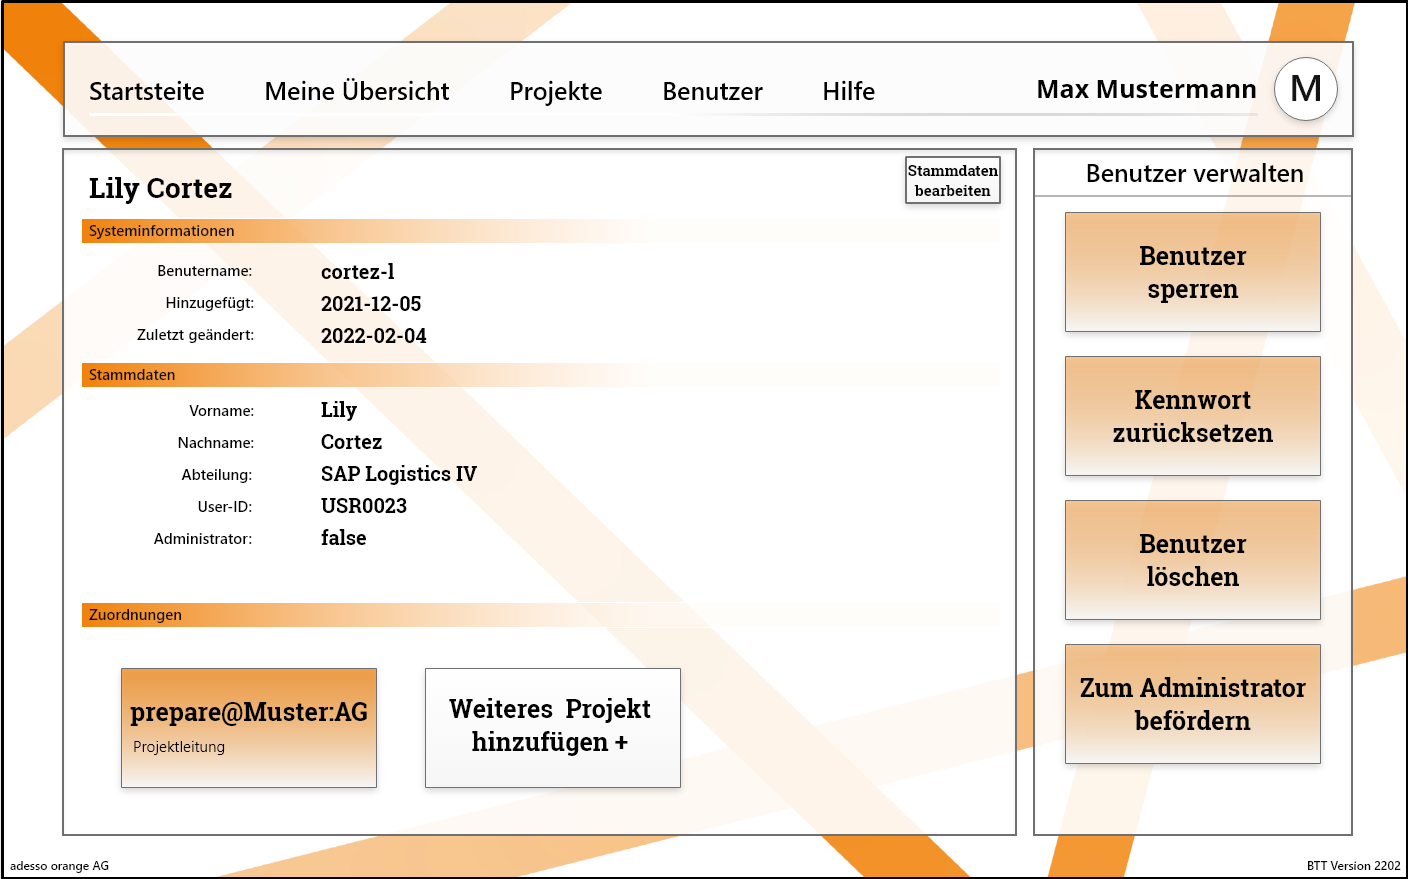
\includegraphics[scale=0.35]{./Prototyp/043_Benutzer verwalten.png}
    \caption[Prototyp: Benutzerverwaltung]{Benutzerverwaltung}
    \label{fig:Benutzerverwaltung}
\end{figure}
Aus der in Abbildung \ref{fig:Benutzerverwaltung} dargestellten Ansicht lassen sich die Stammdaten des Benutzers bearbeiten, der Zugang sperren, das Kennwort zurücksetzen, sowie den Benutzern zu weiteren Projekten hinzuzufügen. Ebenfalls besteht die Möglichkeit, den Benutzer zu einem Administrator zu befördern.
\vspace{2em}
\\\emph{Zur verbesserten Anschauung sind die Darstellungen des Prototypen ebenfalls im Verzeichnis ./Prototyp/ dieser Arbeit abgelegt.}